\documentclass{winnower}
\usepackage[table,xcdraw]{xcolor}

\begin{document}

\title{Classification Engine for Pokemon Types}

\author{Devvrat Raghav}
\affil{Economics Department, Ashoka University}
\author{Aditya Singh}
\affil{Computer Science Department, Ashoka University}

\date{}

\maketitle

\begin{abstract}

\end{abstract}


%-------------------------------------------------%
\section{Introduction}
%-------------------------------------------------%

Pokemon is a popular series of role-playing video games where players inhabit a fictional world filled with magical creatures called Pokemon (short for pocket-monsters). Introduced in 1995 with a set of 151 Pokemon, the Pokemon universe has since grown to contain 890 distinct species, several of which have regional variants. Each Pokemon has a Primary type that can be one of eighteen categories, such as Fire, Water, Dragon etc. Many Pokemon also have a distinct secondary type, drawn from the same set of eighteen types. Thus, a Pokemon X can be Water-type, while Pokemon Y can be both Ice and Flying type. \\



Since Pokemon are loosely based on real phenomenon, it is worth asking whether these creatures have some underlying characteristics that could be used to predict their type. One approach could be using a Pokemon's biological traits as a predictors, akin to the practice of classifying animals in Ecology. We adopt two variations of this approach, one based on image data and the other based on text. The image-based approach relies on a Pokemon's official artwork as the input feature set, whereas the text-based approach leverages a textual account of the Pokemon's biology and a curated set of moves that act as an extension of the biological description.



%-------------------------------------------------%
\section{Related Works}
%-------------------------------------------------%

Existing literature in this area is both sparse and recent. Kirkham (2016) separately deployed XGBoost and a Deep Neural Network to predict Pokemon type(s), using features like Egg Groups, Gender Ratio and a Pokemon's base stats. Similarly, De Dios Santos (2016) passed Pokemon images through a Deep Neural Network to to predict their type(s). \\

Much of the research in this field, however, has been oriented towards identifying the optimal strategy for Pokemon battles.\textsuperscript{[1][2][3][4]} Moreover, there have also been attempts to create new Pokemon designs through GANs. Nonetheless, to the best of our knowledge, there has been no other attempt to predict a Pokemon's type(s) using the non-image features we have selected for this paper.

% \begin{equation}
% \Delta =\sum_{i=1}^N w_i (x_i - \bar{x})^2 
% \label{eqn:eq1}
% \end{equation}
%-------------------------------------------------%
\section{Data}
%-------------------------------------------------%
\subsection{Biological Descriptions}
%-------------------------------------------------%	 

The biological descriptions for Pokemon were sourced from Bulbapedia, where the \emph{Biology} section describes the Pokemon's official artwork using physiological nomenclature. This applies to both organism-based and object-inspired Pokemon. In addition, it contains brief snippets about the Pokemon's general disposition, such as their attitude, habitat or special powers. For instance, Gardevoir's biological description reads:

\begin{figure*}
\begin{center}
\begin{minipage}[b]{0.3\textwidth}
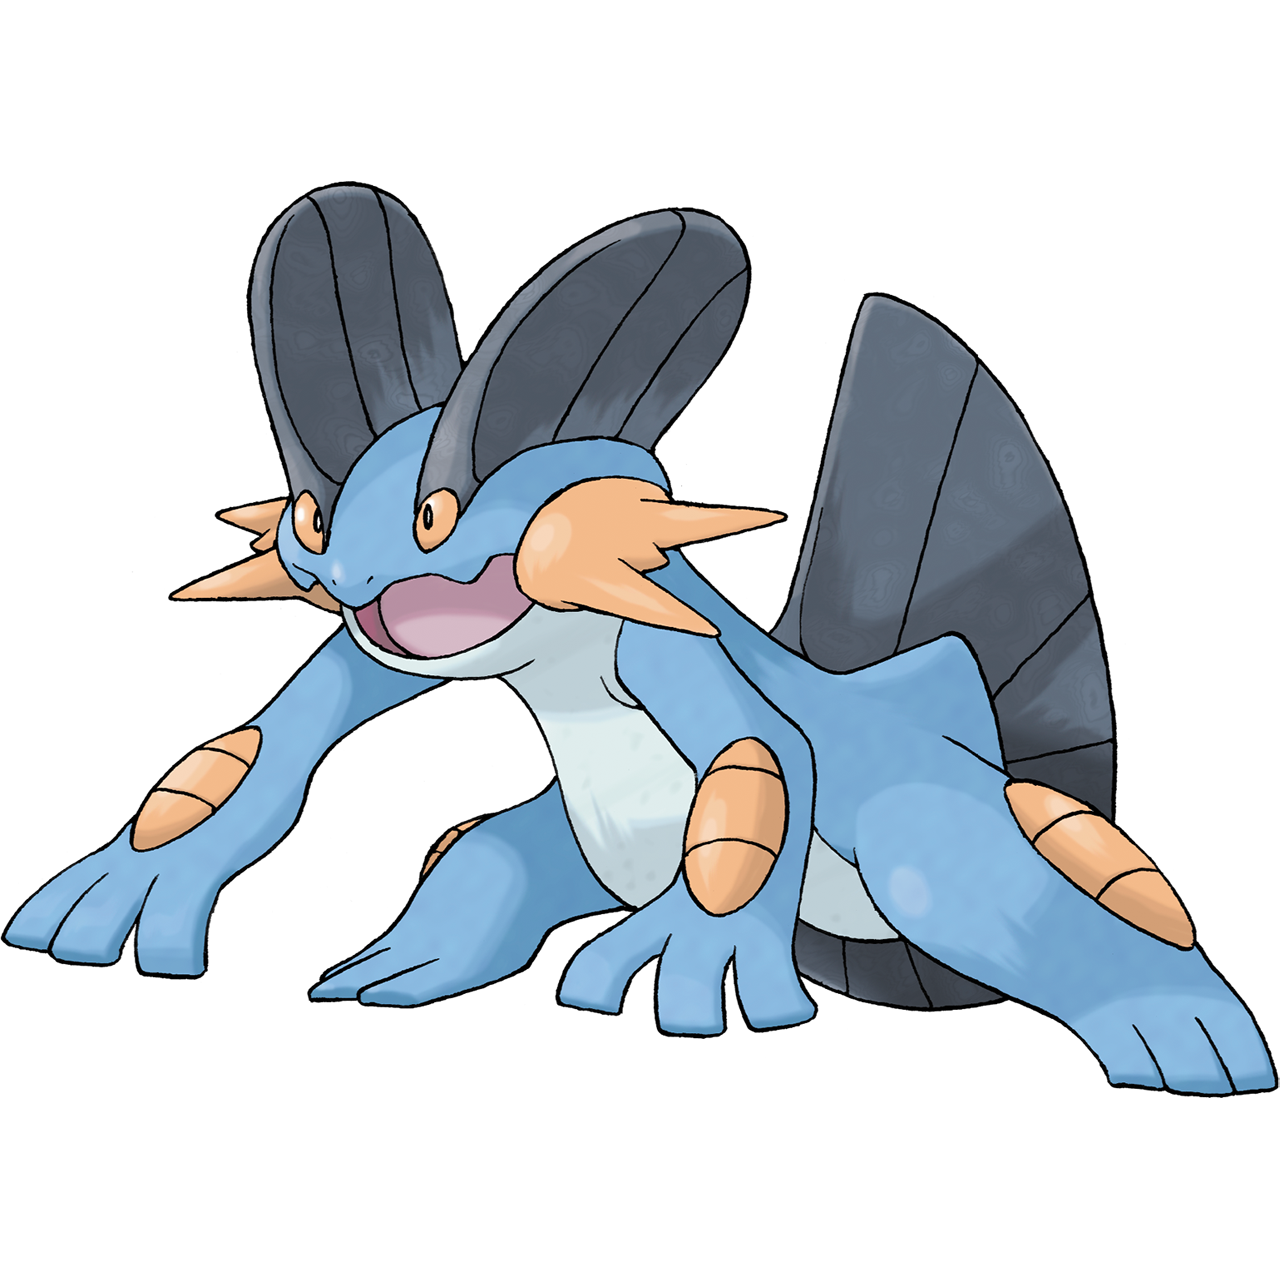
\includegraphics[scale=0.1]{Swampert.jpg}\vspace{0cm}
\caption
{Swampert (Water / Ground type)}
\end{minipage}
\hfill
\begin{minipage}[b]{0.3\textwidth}

\includegraphics[scale=0.1]{Pikachu.jpg}\vspace{0cm}
\caption
{Pikachu (Electric type) }
\end{minipage}
\hfill
\begin{minipage}[b]{0.3\textwidth}

\includegraphics[scale=0.1]{Gardevoir.jpg}\vspace{0cm}
\caption
{Gardevoir (Psychic / Fairy type)}
\end{minipage}
\end{center}
\end{figure*}


\begin{verbatim}
    Gardevoir is a bipedal, humanoid Pokemon whose body resembles a flowing gown. Most of 
    its body is white, but its hair, arms, and the underside of its gown are green. Its 
    hair curls over its face and down the sides of its head. Behind its red eyes are short
    spikes, resembling a masquerade mask. It has long arms with three fingers on each hand 
    and slender white legs. A red, fin-like horn extends from its chest, and a shorter, 
    more rounded horn extends from the back.A band of green on its chest extends to the 
    center of the front horn and connects to its sleeve-like arms.
    Gardevoir is able to see the future using its psychic powers. Additionally, it is able 
    to create small black holes, distort dimensions, and support itself without feeling
    the pull of gravity. Its power reaches its peak when protecting its Trainer, whom 
    it will protect with its life. This Pokemon inhabits urban areas.
\end{verbatim}
\\
This data was mined and initially stored as text interspersed with HTML tags. It was then cleaned using regular expressions. All HTML tags, along with punctuation, were stripped away. The resulting text was then converted into TF-IDF features. Since this resulted in a large sparse matrix of size $802 \times 9100$, the TF-IDF matrix was put through Latent Semantic Analysis (LSA). As a result, the dimensionality of each Pokemon's biology was reduced to 750 components, resulting in an $802 \times 750$ feature matrix. Both the TF-IDF vectorization and LSA was carried out through the \emph{scikit-learn} module in Python.
%-------------------------------------------------%
\subsection{Moves Learnt}
%-------------------------------------------------%	 

It was apparent that the biological descriptions on Bulbapedia, while extensive and accurate, were not detailed enough to account for the abilities of Pokemon. Specifically, each Pokemon is able to use dozens of moves that are sometimes exclusive to its species. More importantly, the kind of moves that a Pokemon can learn are informed by its biology and underlying characteristics, which we hypothesised as also being potential predictors of its type(s). \\



As a result, we used our domain knowledge to curate a set of 20 moves that would augment the Pokemon's biology. These moves were chosen on the basis of their (i) exclusivity to certain groups of Pokemon and (ii) biological prerequisites. Moves that could only be learnt by Pokemon who shared a common biological feature were preferred, where the feature is not just limited to a Pokemon's outwardly appearance or limbs. Additionally, moves that were teachable through Technical Machines (TMs) or Move Tutors were preferred, since any Pokemon that is capable of learning this move can learn it through these methods, even if they don't learn it by levelling up. Since the move places the same physiological constraints on a Pokemon irrespective of where it was learnt from, choosing such moves is no worse than picking their counterparts that can only be learnt via levelling up.\\

For instance, the move High Jump Kick was selected because it highlights a Pokemon's jumping and kicking ability that may not be captured in its Bulbapedia description. Similarly, moves like Flame Charge and Draco Meteor were chosen because they had clear \textit{de facto} prerequisites, namely being able to organically create flames and summon the atmosphere's latent draconic energy, respectively. \\

Stated otherwise, if a Pokemon is able to learn Flame Charge - primarily \textit{Fire-type} Pokemon - then its underlying characteristics are different from Pokemon that cannot learn it, such as \textit{Water-type} Pokemon. Given this, these moves are not just additional features, but an extension of a Pokemon's biological traits. In other words, they carry a lot of information. We represent them in the form of a binary vector of length 20.


%-------------------------------------------------%
\subsection{Images}
%-------------------------------------------------%

The images of the official artwork of the pokemons was taken from Bulbapedia as well

%%%%%%%%%%%%%%%%%%%%%%%%%%%%%%%%%%%%%%%%%%%%%%%%

%%%%%%%%%%%%%%%%%%%%%%%%%%%%%%%%%%%%%%%%%%%%%%%%

%-------------------------------------------------%

% Table 2
% Please add the following required packages to your document preamble:
% If you use beamer only pass "xcolor=table" option, i.e. \documentclass[xcolor=table]{beamer}

%-------------------------------------------------%
\subsection{Pokemon Type(s)}
%-------------------------------------------------%	 

Each Pokemon's type(s) were gotten from a dataset that was independently created specifically for this project. Types were divided into two columns - Primary and Secondary. These were then encoded into a binary vector of length 18, corresponding to the number of possible types. Two such encodings were created, one for a Pokemon's Primary type and one for its complete typing (Primary and Secondary). Thus, a Normal/Flying-type Pokemon would be represented as -
\begin{center}
    

                      $[ 1, 0, 1, 0, 0, 0, 0, 0, 0, 0, 0, 0, 0, 0, 0, 0, 0, 0] $\\
                      \end{center}
where 1 indicates presence of a type label and 0 indicates the absence of that label. The need for two encodings is explained below in the next section.

%-------------------------------------------------%
\section{Classification Methods }
%-------------------------------------------------%

We address this classification problem in two ways. First, we treat it as a multi-class classification problem, where only the Primary type label of a Pokemon is to be predicted. This was the purpose behind creating a separate encoding for a Pokemon's Primary type. Second, we treat it as a multi-class, multi-label classification problem, where all type(s) labels of a Pokemon are to be predicted.

It is noteworthy that the second problem is neither truly multi-class, nor multi-label. After all, some Pokemon can have two simultaneous type labels, which makes the labels non-mutually-exclusive. However, there can be no more than two type labels for any Pokemon, which means that the presence of any type label X is not truly independent of another type. Essentially, the number of labels to be predicted lies in the range $[1, 2]$. This means that multi-label methods, which are designed to output any number of concurrent type labels, are not best-suited to this problem.

%-------------------------------------------------%
\subsection{Predicting Primary Type}
%-------------------------------------------------%	 
This is handled by different networks for text-based and image-based approaches, each of which is described in its own subsection.
%-------------------------------------------------%
\subsubsection{Neural Network}
%-------------------------------------------------%	 
The shallow Neural Network has $64$ nodes in the hidden layer and $18$ nodes in the output layer, corresponding to the number of target classes. Activation for the hidden layer is handled by the $Relu$ function, chosen for its computational simplicity. Meanwhile, the output layer uses a $Softmax$ activation function, since only a singular type label is desired as the network's output. For any given label $i$, the activation function is defined as:
\begin{equation*}
S(y_{i}) = \frac{e^{y_{i}}}{\sum_{j\neq i}^{18} e^{y_{j}}}
\end{equation*}Given the multi-class nature of the problem, the loss function of choice was \emph{Categorical Cross-Entropy}. Since \textit{Categorical Cross-Entropy} calculates the log-loss just for the target label of interest, its penalty on the $Softmax$ activation's output increases if the output probability is less-concentrated in the correct target label. Consequently, the network should learn to readjust weights such that the correct label is much more likely to be predicted, which naturally makes other (incorrect) labels less likely to be chosen. \\

The network was created using \emph{keras} with a \emph{tensorflow} backend and trained for $40$ epochs on eighty percent of the total sample ($802$ observations), which amounted to $641$ training examples. Optimisation was handled by $Adam$. \\

This network is run for three different variations of inputs. In its first variation, it takes only the reduced-dimension representation of the biology, i.e. has an input feature vector of length $750$. In its second variation, it takes both the dense representation and binary move vector as inputs, thereby making the input dimension $641 \times 770$. In its final variation, the network takes just the move vector as an input. The target labels are one-hot encoded.

%-------------------------------------------------%
\subsubsection{k-Nearest Neighbours}
%-------------------------------------------------%	 
The second classification algorithm used was k-Nearest Neighbours, where a grid search was conducted to find the optimal size for $k$.  Different values of $k$ were compared using the $accuracy$ metric on test data, after which $k = 3$ was chosen. This algorithm was trained on the same three variations of the input data as the Neural Network.

%-------------------------------------------------%
\subsubsection{Convolutional Neural Network}
%-------------------------------------------------%	 
Lorem ipsum dolor sit amet, consectetur adipiscing elit. Suspendisse accumsan magna est, quis elementum leo laoreet eu. Donec sollicitudin elit non massa venenatis, in viverra dolor sagittis. Maecenas ac justo pulvinar, consectetur mauris hendrerit, vulputate lacus. Etiam tristique sapien quis sem commodo, et eleifend tortor viverra. In hac habitasse platea dictumst. Phasellus vel tempus risus, sit amet consectetur massa. Duis rutrum lectus eu ligula egestas iaculis. Sed condimentum, ipsum in dignissim condimentum, nisi turpis blandit massa, et aliquam magna ligula eget lacus. Donec ac eleifend nulla, quis cursus nisi. 

%-------------------------------------------------%
\subsection{Predicting Multiple Types}
%-------------------------------------------------%	 

Since this is effectively a constrained multi-label classification problem, the algorithms of choice here are somewhat different variations of the previous ones.

%-------------------------------------------------%
\subsubsection{Neural Network}
%-------------------------------------------------%	 
This shallow neural network is mostly similar to the previous design. There are $18$ output nodes and $64$ nodes in the hidden layer, which use a $Relu$ activation function. Once again, activation in the output layer is handled by the$Softmax$ function.

The main change is the choice of loss function, with \emph{Binary Cross-Entropy} being selected for this network. Since \emph{Binary Cross-Entropy} essentially applies Cross-Entropy loss to each type label $i$ and takes the sum, it allows multiple labels to co-occur. At the same time, the $Softmax$ activation squashes the probability into one or a few type labels. This creates a somewhat-adversarial system of counterbalance that allows both one and two type labels to be predicted for different Pokemon. 

Like all previous classifiers, this network is trained on the same three variations of input features. However, the target labels use the second encoding outlined in Section $3$, i.e. a binary string of length $18$ with multiple type labels encoded as $1$. 

%-------------------------------------------------%
\subsubsection{Multi-Label k-Nearest Neighbours}
%-------------------------------------------------%	 
Multi-label k-Nearest Neighbours, henceforth referred to as MLkNN, is an adaptation of k-Nearest Neighbours designed for multi-label classification.[5] For every test instance $l$, the algorithm finds its k-nearest neighbours, then applies uses the \textit{maximum a posteriori} principle to compute the class label(s) for instance $l$ based on the class label information of its neighbours.

The algorithm takes two parameters $k$ and $s$, which correspond to number of nearest neighbours and smoothing factor, respectively. A grid search was employed to find the optimal value for both, and it was found that $k = 1$ and $s = 1.0$ were optimal for predicting Pokemon type labels. It was trained on all three variations of input features, and returned a binary vector of length $18$ as the output, where $1$ denoted presence of that type label and $0$ denoted its absence.

%-------------------------------------------------%
\subsubsection{Binary Relevance - Logistic Regression}
%-------------------------------------------------%	 
Binary Relevance is a one-versus-Rest scheme used for multi-label classification where, for $q$ class labels, $q$ independent classifiers are created to predict the presence of individual class labels. In this case, a total of $18$ Logistic Regression classifiers [$c_{1}, c_{2}, ..., c_{18}$] are trained on all three variations of the input features. Using grid search, the regularisation parameter $c$ was set to $1.0$, and the solver used was $LBFGS$.

Notably, since each classifier is independent, this approach fails to account for correlation between Pokemon type labels, which is a major shortcoming because Pokemon types observe a non-random distribution of secondary type labels ($type2$), when conditioned on the primary label ($type1$) and otherwise. 

%-------------------------------------------------%
\subsubsection{Convolutional Neural Network}
%-------------------------------------------------%	 
Multi-label k-Nearest Neighbours, henceforth referred to as MLkNN, is an adaptation of k-Nearest Neighbours designed for multi-label classification.[5] For every test instance $l$, the algorithm finds its k-nearest neighbours, then applies uses the \textit{maximum a posteriori} principle to compute the class label(s) for instance $l$ based on the class label information of its neighbours.

The algorithm takes two parameters $k$ and $s$, which correspond to number of nearest neighbours and smoothing factor, respectively. A grid search was employed to find the optimal value for both, and it was found that $k = 1$ and $s = 1.0$ were optimal for predicting Pokemon type labels. It was trained on all three variations of input features, and returned a binary vector of length $18$ as the output, where $1$ denoted presence of that type label and $0$ denoted its absence.

%-------------------------------------------------%
\section{Results }
%-------------------------------------------------%
Before the results are analysed, it is essential to observe the distribution of the type labels within the sample of $802$ Pokemon. This allows us to set \textit{a priori} expectations about the likelihood of overfitting, based on the class imbalance within the output labels, or lack thereof. Hence, these distributions are computed separately for the multi-class and multi-label type-classification problems and presented below in the histograms:

\begin{figure}[!htb]%
\centering
\subfigure[A]{%
\label{fig:first}%
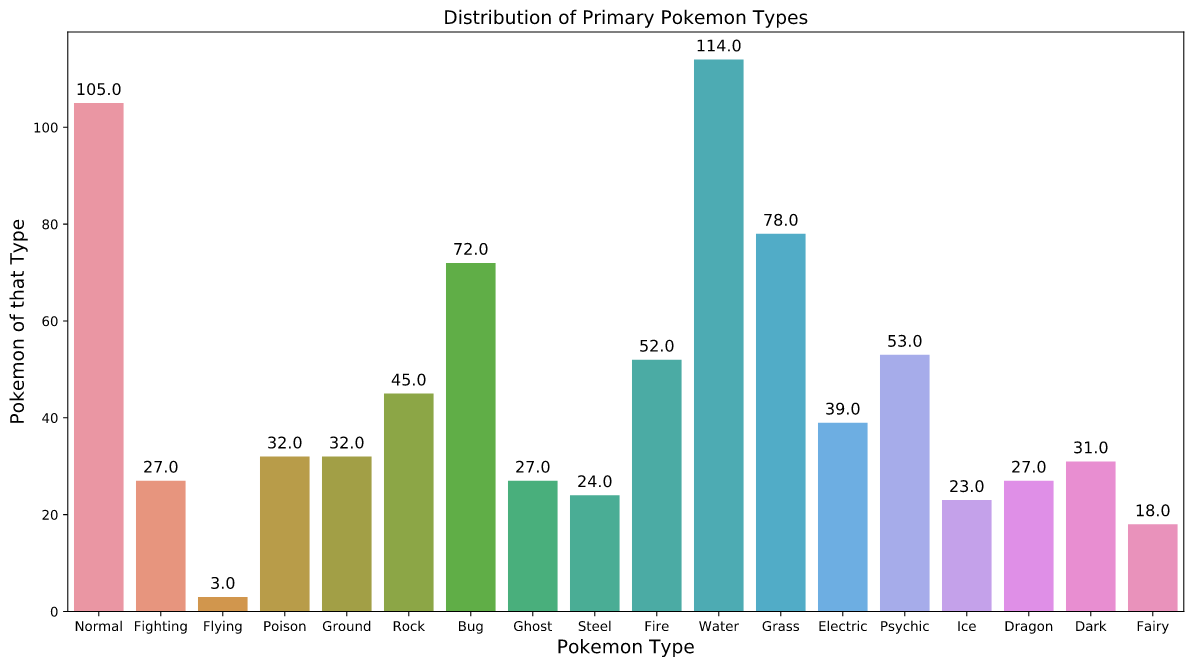
\includegraphics[height=2.4 in]{primTypeDist.png}}
\qquad
\subfigure[B]{%
\label{fig:second}%
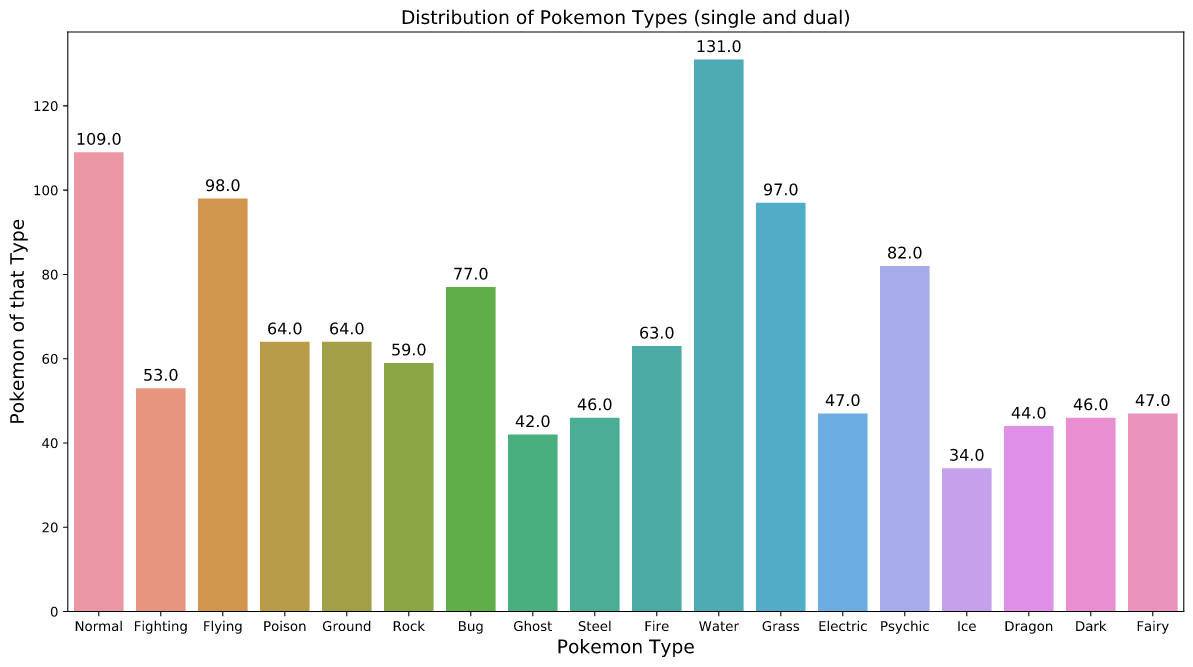
\includegraphics[height=2.4 in]{dualTypeDist.png}}
\caption{A) Distribution of types in the Primary slot \\ B) Distribution of Pokemon types (Primary and Secondary combined) }


\end{figure}

It is clear that the sample of Primary types is imbalanced, since the Water and Normal labels together represent about 25\% of the data. Likewise, the Bug and Grass typings are also prominent, while several type labels occur very infrequently, with Flying being the rarest Primary type (only $3$ out of $802$ Pokemon have this label). 

On the other hand, the distribution of all type labels for each Pokemon - as visualised in histogram B - is relatively more even. It is notable that the previously rare Flying and Steel types become more prominent in this case, which makes this distribution of type labels more \textit{heavy-tailed} than the previous one. 

Having done this, we briefly outline the performance metrics used to compare classifiers in both the Primary and Multi-Type classification problems:

\begin{enumerate}
\item  Precision - The macro-average of Precision is used, i.e. Precision is calculated for each type label $i$ and the mean across all type labels is used.
\item Recall - The macro-average of Recall is used, just like the Precision metric.
\item F-Score - The F1-Score is computed for each label $i$ and a weighted average is taken. The weight used for any label $i$ is the \textit{support} for that label.
\item Accuracy - In the Primary-type case, this is simply defined as the the proportion of types correctly predicted. In the Multi-type case, this computes the subset accuracy, i.e. the proportion of \textit{correct} labels to the total number of labels (predicted and actual) for every example $l$, and then takes the average.
\item Top-K Accuracy - For each example $l$, this indicator function returns a $1$ if the true type label(s) is in the top-k predictions of the classifier. In the Primary-type case, $k$ is set to $2$, meaning that even if the classifier predicts the true label (say, Ice-type) as the second-most likely label, then this returns a $1$ for that example. However, it returns a $0$ if the true label is outside the top $k$ predictions. In the Multi-type case, $k$ is set to $3$, since up to $2$ types can be simultaneously predicted. Thus, using a window of top-3 predictions allows us to see whether the classifier was close to predicting all type(s) correctly.  The indicator function is averaged across all training examples.
\item  Hamming Loss - Used exclusively in the Multi-Type case, where its defined as fraction of type labels that were incorrectly predicted.
\end{enumerate}


%-------------------------------------------------%
\subsection{Performance on Primary Type Classification}
%-------------------------------------------------%

\begin{center}
\begin{tabular}{lccccc} \multicolumn{6}{c}{Table 1 - Performance Measures for Primary Type Classification} \\ \hline
& & & & &  \\
Classifier & Precision & Recall & F-Score & Accuracy & Top-K Accuracy (k=2) \\ \hline
& & & & &  \\
Neural Net (only bio) & 0.44 & 0.31 & 0.30 & 0.48 & 1.0 \\
& & & & &  \\
Neural Net (only moves) & 0.61 & 0.60 & 0.58 & 0.72 & 1.0 \\
& & & & &  \\
Neural Net (bio + moves) & 0.61 & 0.62 & 0.69 & 0.74 & 1.0 \\
& & & & &  \\
k-Nearest Neighbours (only bio) & 0.53 & 0.24 & 0.30 & 0.25 & 1.0 \\
& & & & &  \\
k-NN (w/ moves) & 0.57 & 0.53 & 0.52 & 0.59 & 1.0 \\
& & & & &  \\ \hline
\end{tabular}
\end{center}

From an \textit{accuracy} standpoint, k-Nearest Neighbours, when used only on the LSA representation of Pokemon biology, is the least effective classifier for this purpose. Given its \textit{Accuracy} of 25\%, it is, on average, no better than any naive algorithm that simply classifies every Pokemon as either Water or Normal type. The \textit{recall}, in particular, suffers greatly here as the algorithm very rarely outputs an uncommon type label as the prediction for an unseen Pokemon. The higher \textit{precision} is likely aided by the class imbalance, which allows the dominant class predictions to be accurate 53\% of the time. 

It is interesting then, to see that the performance of k-NN improves markedly across the board once the move vector are included as inputs. \textit{Recall} and \textit{Accuracy} jump to 53\% and 59\% respectively, indicating that the biological descriptions (in dense representation) were insufficient to separate out the different types. Stated otherwise, including moves to extend the biology allows us to saturate the k-NN's predictive power -  previously constrained by the input features. 

In comparison, a Neural Network performs better with every variation of input features, at least from an \textit{Accuracy} and \textit{Recall} perspective. It is able to predict the common types, not just Water and Normal, but also Bug, Grass and Electric. However, performance with just the biological descriptions is not very different from k-NN, since the higher \textit{Recall} must be looked at together with the lower \textit{Precision}. Essentially, the network is predicting the uncommon labels correctly more often, but its predictions for the dominant classes somewhat suffer as a result. This is corroborated by the F-Score, with the neural network's higher F-Score reflecting its ability to predict the less-dominant classes correctly

It is also clear that the move vector is an essential component of the input features, since a network trained only on this $20$ length vector demonstrated superior performance across every metric when compared to its counterpart trained only on the biological descriptions. If anything, the moves are arguably a better dense representation of the Pokemon's biological traits than the Bulbapedia descriptions, at least as inputs for a classifier. It is then unsurprising to see a network trained on both moves and biological description outperform all other classifiers chosen for this task. Achieving category-highest \textit{Accuracy}, \textit{Precision} and \textit{Recall} scores, this network predicts more classes correctly, and its predictions are most likely (relative to others) to be correct.  

%-------------------------------------------------%
\subsection{Performance on Multi-Type Classification}
%-------------------------------------------------%


\begin{center}
\begin{tabular}{lcccccc} \multicolumn{7}{c}{Table 3 - Performance Measures for Multi-Type(s) Classification} \\ \hline
& & & & & & \\
Classifier & Precision & Recall & F-Score & Accuracy & Top-K Accuracy (k=3) & Hamming Loss \\ \hline
& & & & & & \\
Neural Net (only bio) & 0.44 & 0.31 & 0.30 & 0.91 & 1.0 & 0.11 \\
& & & & & & \\
Neural Net (only moves) & 0.44 & 0.75 & 0.66 & 0.95 & 1.0 & 0.078 \\
& & & & & & \\
Neural Net (bio +  moves) & 0.60 & 0.72 & 0.69 & 0.96 & 1.0 & 0.077 \\
& & & & & & \\
ML k-NN (only bio) & 0.53 & 0.24 & 0.30 & 0.31 & 1.0 & 0.08 \\
& & & & & & \\
MLk-NN (w/ moves) & 0.74 & 0.76 & 0.73 & 0.56 & 1.0 & 0.04 \\
& & & & & & \\ \hline
\end{tabular}
\end{center}


% \acknowledgments
% Lorem ipsum dolor sit amet, consectetur adipiscing elit. Suspendisse accumsan magna est, quis elementum leo laoreet eu. Donec sollicitudin elit non massa venenatis, in viverra dolor sagittis. Maecenas ac justo pulvinar, consectetur mauris hendrerit, vulputate lacus. Etiam tristique sapien quis sem commodo, et eleifend tortor viverra.

% \bibliographystyle{abbrvnat}
% \bibliography{winnower_template}

% \appendix


\section{Appendix Heading}
Lorem ipsum dolor sit amet, consectetur adipiscing elit. Suspendisse accumsan magna est, quis elementum leo laoreet eu. Donec sollicitudin elit non massa venenatis, in viverra dolor sagittis. Maecenas ac justo pulvinar, consectetur mauris hendrerit, vulputate lacus. Etiam tristique sapien quis sem commodo, et eleifend tortor viverra. In hac habitasse platea dictumst. Phasellus vel tempus risus, sit amet consectetur massa. Duis rutrum lectus eu ligula egestas iaculis. Sed condimentum, ipsum in dignissim condimentum, nisi turpis blandit massa, et aliquam magna ligula eget lacus. Donec ac eleifend nulla, quis cursus nisi. Lorem ipsum dolor sit amet, consectetur adipiscing elit. Suspendisse accumsan magna est, quis elementum leo laoreet eu. Donec sollicitudin elit non massa venenatis, in viverra dolor sagittis. Maecenas ac justo pulvinar, consectetur mauris hendrerit, vulputate lacus. Etiam tristique sapien quis sem commodo, et eleifend tortor viverra. In hac habitasse platea dictumst. Phasellus vel tempus risus, sit amet consectetur massa. Duis rutrum lectus eu ligula egestas iaculis. Sed condimentum, ipsum in dignissim condimentum, nisi turpis blandit massa, et aliquam magna ligula eget lacus. Donec ac eleifend nulla, quis cursus nisi







\end{document}